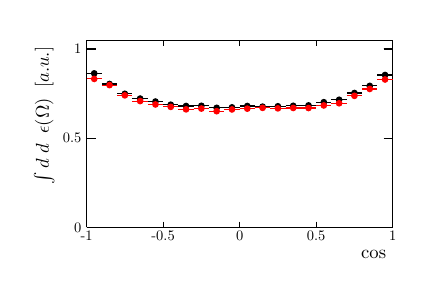
\begin{tikzpicture}
\pgfdeclareplotmark{cross} {
\pgfpathmoveto{\pgfpoint{-0.3\pgfplotmarksize}{\pgfplotmarksize}}
\pgfpathlineto{\pgfpoint{+0.3\pgfplotmarksize}{\pgfplotmarksize}}
\pgfpathlineto{\pgfpoint{+0.3\pgfplotmarksize}{0.3\pgfplotmarksize}}
\pgfpathlineto{\pgfpoint{+1\pgfplotmarksize}{0.3\pgfplotmarksize}}
\pgfpathlineto{\pgfpoint{+1\pgfplotmarksize}{-0.3\pgfplotmarksize}}
\pgfpathlineto{\pgfpoint{+0.3\pgfplotmarksize}{-0.3\pgfplotmarksize}}
\pgfpathlineto{\pgfpoint{+0.3\pgfplotmarksize}{-1.\pgfplotmarksize}}
\pgfpathlineto{\pgfpoint{-0.3\pgfplotmarksize}{-1.\pgfplotmarksize}}
\pgfpathlineto{\pgfpoint{-0.3\pgfplotmarksize}{-0.3\pgfplotmarksize}}
\pgfpathlineto{\pgfpoint{-1.\pgfplotmarksize}{-0.3\pgfplotmarksize}}
\pgfpathlineto{\pgfpoint{-1.\pgfplotmarksize}{0.3\pgfplotmarksize}}
\pgfpathlineto{\pgfpoint{-0.3\pgfplotmarksize}{0.3\pgfplotmarksize}}
\pgfpathclose
\pgfusepathqstroke
}
\pgfdeclareplotmark{cross*} {
\pgfpathmoveto{\pgfpoint{-0.3\pgfplotmarksize}{\pgfplotmarksize}}
\pgfpathlineto{\pgfpoint{+0.3\pgfplotmarksize}{\pgfplotmarksize}}
\pgfpathlineto{\pgfpoint{+0.3\pgfplotmarksize}{0.3\pgfplotmarksize}}
\pgfpathlineto{\pgfpoint{+1\pgfplotmarksize}{0.3\pgfplotmarksize}}
\pgfpathlineto{\pgfpoint{+1\pgfplotmarksize}{-0.3\pgfplotmarksize}}
\pgfpathlineto{\pgfpoint{+0.3\pgfplotmarksize}{-0.3\pgfplotmarksize}}
\pgfpathlineto{\pgfpoint{+0.3\pgfplotmarksize}{-1.\pgfplotmarksize}}
\pgfpathlineto{\pgfpoint{-0.3\pgfplotmarksize}{-1.\pgfplotmarksize}}
\pgfpathlineto{\pgfpoint{-0.3\pgfplotmarksize}{-0.3\pgfplotmarksize}}
\pgfpathlineto{\pgfpoint{-1.\pgfplotmarksize}{-0.3\pgfplotmarksize}}
\pgfpathlineto{\pgfpoint{-1.\pgfplotmarksize}{0.3\pgfplotmarksize}}
\pgfpathlineto{\pgfpoint{-0.3\pgfplotmarksize}{0.3\pgfplotmarksize}}
\pgfpathclose
\pgfusepathqfillstroke
}
\pgfdeclareplotmark{newstar} {
\pgfpathmoveto{\pgfqpoint{0pt}{\pgfplotmarksize}}
\pgfpathlineto{\pgfqpointpolar{44}{0.5\pgfplotmarksize}}
\pgfpathlineto{\pgfqpointpolar{18}{\pgfplotmarksize}}
\pgfpathlineto{\pgfqpointpolar{-20}{0.5\pgfplotmarksize}}
\pgfpathlineto{\pgfqpointpolar{-54}{\pgfplotmarksize}}
\pgfpathlineto{\pgfqpointpolar{-90}{0.5\pgfplotmarksize}}
\pgfpathlineto{\pgfqpointpolar{234}{\pgfplotmarksize}}
\pgfpathlineto{\pgfqpointpolar{198}{0.5\pgfplotmarksize}}
\pgfpathlineto{\pgfqpointpolar{162}{\pgfplotmarksize}}
\pgfpathlineto{\pgfqpointpolar{134}{0.5\pgfplotmarksize}}
\pgfpathclose
\pgfusepathqstroke
}
\pgfdeclareplotmark{newstar*} {
\pgfpathmoveto{\pgfqpoint{0pt}{\pgfplotmarksize}}
\pgfpathlineto{\pgfqpointpolar{44}{0.5\pgfplotmarksize}}
\pgfpathlineto{\pgfqpointpolar{18}{\pgfplotmarksize}}
\pgfpathlineto{\pgfqpointpolar{-20}{0.5\pgfplotmarksize}}
\pgfpathlineto{\pgfqpointpolar{-54}{\pgfplotmarksize}}
\pgfpathlineto{\pgfqpointpolar{-90}{0.5\pgfplotmarksize}}
\pgfpathlineto{\pgfqpointpolar{234}{\pgfplotmarksize}}
\pgfpathlineto{\pgfqpointpolar{198}{0.5\pgfplotmarksize}}
\pgfpathlineto{\pgfqpointpolar{162}{\pgfplotmarksize}}
\pgfpathlineto{\pgfqpointpolar{134}{0.5\pgfplotmarksize}}
\pgfpathclose
\pgfusepathqfillstroke
}
\definecolor{c}{rgb}{1,1,1};
\draw [color=c, fill=c] (5.1,3.20034) rectangle (9.9,6.21242);
\draw [color=c, fill=c] (5.772,3.68227) rectangle (9.66,6.06181);
\definecolor{c}{rgb}{0,0,0};
\draw [c] (5.772,3.68227) -- (5.772,6.06181) -- (9.66,6.06181) -- (9.66,3.68227) -- (5.772,3.68227);
\draw [c,line width=0.4] (5.8692,5.62691) -- (5.8692,5.63874);
\draw [c,line width=0.4] (5.8692,5.63874) -- (5.8692,5.65057);
\draw [c,line width=0.4] (5.772,5.63874) -- (5.8692,5.63874);
\draw [c,line width=0.4] (5.8692,5.63874) -- (5.9664,5.63874);
\foreach \P in {(5.8692,5.63874)}{\draw[mark options={color=c,fill=c},mark size=2.402402pt,mark=*,mark size=1pt] plot coordinates {\P};}
\draw [c,line width=0.4] (6.0636,5.49391) -- (6.0636,5.50447);
\draw [c,line width=0.4] (6.0636,5.50447) -- (6.0636,5.51502);
\draw [c,line width=0.4] (5.9664,5.50447) -- (6.0636,5.50447);
\draw [c,line width=0.4] (6.0636,5.50447) -- (6.1608,5.50447);
\foreach \P in {(6.0636,5.50447)}{\draw[mark options={color=c,fill=c},mark size=2.402402pt,mark=*,mark size=1pt] plot coordinates {\P};}
\draw [c,line width=0.4] (6.258,5.36949) -- (6.258,5.37943);
\draw [c,line width=0.4] (6.258,5.37943) -- (6.258,5.38937);
\draw [c,line width=0.4] (6.1608,5.37943) -- (6.258,5.37943);
\draw [c,line width=0.4] (6.258,5.37943) -- (6.3552,5.37943);
\foreach \P in {(6.258,5.37943)}{\draw[mark options={color=c,fill=c},mark size=2.402402pt,mark=*,mark size=1pt] plot coordinates {\P};}
\draw [c,line width=0.4] (6.4524,5.30891) -- (6.4524,5.31858);
\draw [c,line width=0.4] (6.4524,5.31858) -- (6.4524,5.32825);
\draw [c,line width=0.4] (6.3552,5.31858) -- (6.4524,5.31858);
\draw [c,line width=0.4] (6.4524,5.31858) -- (6.5496,5.31858);
\foreach \P in {(6.4524,5.31858)}{\draw[mark options={color=c,fill=c},mark size=2.402402pt,mark=*,mark size=1pt] plot coordinates {\P};}
\draw [c,line width=0.4] (6.6468,5.27176) -- (6.6468,5.2813);
\draw [c,line width=0.4] (6.6468,5.2813) -- (6.6468,5.29083);
\draw [c,line width=0.4] (6.5496,5.2813) -- (6.6468,5.2813);
\draw [c,line width=0.4] (6.6468,5.2813) -- (6.744,5.2813);
\foreach \P in {(6.6468,5.2813)}{\draw[mark options={color=c,fill=c},mark size=2.402402pt,mark=*,mark size=1pt] plot coordinates {\P};}
\draw [c,line width=0.4] (6.8412,5.23139) -- (6.8412,5.24083);
\draw [c,line width=0.4] (6.8412,5.24083) -- (6.8412,5.25027);
\draw [c,line width=0.4] (6.744,5.24083) -- (6.8412,5.24083);
\draw [c,line width=0.4] (6.8412,5.24083) -- (6.9384,5.24083);
\foreach \P in {(6.8412,5.24083)}{\draw[mark options={color=c,fill=c},mark size=2.402402pt,mark=*,mark size=1pt] plot coordinates {\P};}
\draw [c,line width=0.4] (7.0356,5.21504) -- (7.0356,5.22447);
\draw [c,line width=0.4] (7.0356,5.22447) -- (7.0356,5.2339);
\draw [c,line width=0.4] (6.9384,5.22447) -- (7.0356,5.22447);
\draw [c,line width=0.4] (7.0356,5.22447) -- (7.1328,5.22447);
\foreach \P in {(7.0356,5.22447)}{\draw[mark options={color=c,fill=c},mark size=2.402402pt,mark=*,mark size=1pt] plot coordinates {\P};}
\draw [c,line width=0.4] (7.23,5.21749) -- (7.23,5.22703);
\draw [c,line width=0.4] (7.23,5.22703) -- (7.23,5.23658);
\draw [c,line width=0.4] (7.1328,5.22703) -- (7.23,5.22703);
\draw [c,line width=0.4] (7.23,5.22703) -- (7.3272,5.22703);
\foreach \P in {(7.23,5.22703)}{\draw[mark options={color=c,fill=c},mark size=2.402402pt,mark=*,mark size=1pt] plot coordinates {\P};}
\draw [c,line width=0.4] (7.4244,5.19173) -- (7.4244,5.20122);
\draw [c,line width=0.4] (7.4244,5.20122) -- (7.4244,5.21071);
\draw [c,line width=0.4] (7.3272,5.20122) -- (7.4244,5.20122);
\draw [c,line width=0.4] (7.4244,5.20122) -- (7.5216,5.20122);
\foreach \P in {(7.4244,5.20122)}{\draw[mark options={color=c,fill=c},mark size=2.402402pt,mark=*,mark size=1pt] plot coordinates {\P};}
\draw [c,line width=0.4] (7.6188,5.19782) -- (7.6188,5.20735);
\draw [c,line width=0.4] (7.6188,5.20735) -- (7.6188,5.21689);
\draw [c,line width=0.4] (7.5216,5.20735) -- (7.6188,5.20735);
\draw [c,line width=0.4] (7.6188,5.20735) -- (7.716,5.20735);
\foreach \P in {(7.6188,5.20735)}{\draw[mark options={color=c,fill=c},mark size=2.402402pt,mark=*,mark size=1pt] plot coordinates {\P};}
\draw [c,line width=0.4] (7.8132,5.21472) -- (7.8132,5.22439);
\draw [c,line width=0.4] (7.8132,5.22439) -- (7.8132,5.23406);
\draw [c,line width=0.4] (7.716,5.22439) -- (7.8132,5.22439);
\draw [c,line width=0.4] (7.8132,5.22439) -- (7.9104,5.22439);
\foreach \P in {(7.8132,5.22439)}{\draw[mark options={color=c,fill=c},mark size=2.402402pt,mark=*,mark size=1pt] plot coordinates {\P};}
\draw [c,line width=0.4] (8.0076,5.20692) -- (8.0076,5.21648);
\draw [c,line width=0.4] (8.0076,5.21648) -- (8.0076,5.22604);
\draw [c,line width=0.4] (7.9104,5.21648) -- (8.0076,5.21648);
\draw [c,line width=0.4] (8.0076,5.21648) -- (8.1048,5.21648);
\foreach \P in {(8.0076,5.21648)}{\draw[mark options={color=c,fill=c},mark size=2.402402pt,mark=*,mark size=1pt] plot coordinates {\P};}
\draw [c,line width=0.4] (8.202,5.21158) -- (8.202,5.22108);
\draw [c,line width=0.4] (8.202,5.22108) -- (8.202,5.23059);
\draw [c,line width=0.4] (8.1048,5.22108) -- (8.202,5.22108);
\draw [c,line width=0.4] (8.202,5.22108) -- (8.2992,5.22108);
\foreach \P in {(8.202,5.22108)}{\draw[mark options={color=c,fill=c},mark size=2.402402pt,mark=*,mark size=1pt] plot coordinates {\P};}
\draw [c,line width=0.4] (8.3964,5.21763) -- (8.3964,5.22708);
\draw [c,line width=0.4] (8.3964,5.22708) -- (8.3964,5.23653);
\draw [c,line width=0.4] (8.2992,5.22708) -- (8.3964,5.22708);
\draw [c,line width=0.4] (8.3964,5.22708) -- (8.4936,5.22708);
\foreach \P in {(8.3964,5.22708)}{\draw[mark options={color=c,fill=c},mark size=2.402402pt,mark=*,mark size=1pt] plot coordinates {\P};}
\draw [c,line width=0.4] (8.5908,5.22277) -- (8.5908,5.2322);
\draw [c,line width=0.4] (8.5908,5.2322) -- (8.5908,5.24164);
\draw [c,line width=0.4] (8.4936,5.2322) -- (8.5908,5.2322);
\draw [c,line width=0.4] (8.5908,5.2322) -- (8.688,5.2322);
\foreach \P in {(8.5908,5.2322)}{\draw[mark options={color=c,fill=c},mark size=2.402402pt,mark=*,mark size=1pt] plot coordinates {\P};}
\draw [c,line width=0.4] (8.7852,5.26319) -- (8.7852,5.27274);
\draw [c,line width=0.4] (8.7852,5.27274) -- (8.7852,5.28229);
\draw [c,line width=0.4] (8.688,5.27274) -- (8.7852,5.27274);
\draw [c,line width=0.4] (8.7852,5.27274) -- (8.8824,5.27274);
\foreach \P in {(8.7852,5.27274)}{\draw[mark options={color=c,fill=c},mark size=2.402402pt,mark=*,mark size=1pt] plot coordinates {\P};}
\draw [c,line width=0.4] (8.9796,5.29385) -- (8.9796,5.30347);
\draw [c,line width=0.4] (8.9796,5.30347) -- (8.9796,5.31309);
\draw [c,line width=0.4] (8.8824,5.30347) -- (8.9796,5.30347);
\draw [c,line width=0.4] (8.9796,5.30347) -- (9.0768,5.30347);
\foreach \P in {(8.9796,5.30347)}{\draw[mark options={color=c,fill=c},mark size=2.402402pt,mark=*,mark size=1pt] plot coordinates {\P};}
\draw [c,line width=0.4] (9.174,5.37964) -- (9.174,5.3896);
\draw [c,line width=0.4] (9.174,5.3896) -- (9.174,5.39955);
\draw [c,line width=0.4] (9.0768,5.3896) -- (9.174,5.3896);
\draw [c,line width=0.4] (9.174,5.3896) -- (9.2712,5.3896);
\foreach \P in {(9.174,5.3896)}{\draw[mark options={color=c,fill=c},mark size=2.402402pt,mark=*,mark size=1pt] plot coordinates {\P};}
\draw [c,line width=0.4] (9.3684,5.46945) -- (9.3684,5.47997);
\draw [c,line width=0.4] (9.3684,5.47997) -- (9.3684,5.49049);
\draw [c,line width=0.4] (9.2712,5.47997) -- (9.3684,5.47997);
\draw [c,line width=0.4] (9.3684,5.47997) -- (9.4656,5.47997);
\foreach \P in {(9.3684,5.47997)}{\draw[mark options={color=c,fill=c},mark size=2.402402pt,mark=*,mark size=1pt] plot coordinates {\P};}
\draw [c,line width=0.4] (9.5628,5.60608) -- (9.5628,5.61823);
\draw [c,line width=0.4] (9.5628,5.61823) -- (9.5628,5.63039);
\draw [c,line width=0.4] (9.4656,5.61823) -- (9.5628,5.61823);
\draw [c,line width=0.4] (9.5628,5.61823) -- (9.66,5.61823);
\foreach \P in {(9.5628,5.61823)}{\draw[mark options={color=c,fill=c},mark size=2.402402pt,mark=*,mark size=1pt] plot coordinates {\P};}
\draw [c,line width=0.4] (5.772,3.68227) -- (9.66,3.68227);
\draw [anchor= east] (9.66,3.34492) node[scale=0.672711, rotate=0]{$\cos\thetamu$};
\draw [c,line width=0.4] (5.772,3.75546) -- (5.772,3.68227);
\draw [c,line width=0.4] (6.744,3.75546) -- (6.744,3.68227);
\draw [c,line width=0.4] (7.716,3.75546) -- (7.716,3.68227);
\draw [c,line width=0.4] (8.688,3.75546) -- (8.688,3.68227);
\draw [c,line width=0.4] (9.66,3.75546) -- (9.66,3.68227);
\draw [anchor=base] (5.772,3.51962) node[scale=0.52322, rotate=0]{-1};
\draw [anchor=base] (6.744,3.51962) node[scale=0.52322, rotate=0]{-0.5};
\draw [anchor=base] (7.716,3.51962) node[scale=0.52322, rotate=0]{0};
\draw [anchor=base] (8.688,3.51962) node[scale=0.52322, rotate=0]{0.5};
\draw [anchor=base] (9.66,3.51962) node[scale=0.52322, rotate=0]{1};
\draw [c,line width=0.4] (5.772,6.06181) -- (9.66,6.06181);
\draw [c,line width=0.4] (5.772,5.98862) -- (5.772,6.06181);
\draw [c,line width=0.4] (6.744,5.98862) -- (6.744,6.06181);
\draw [c,line width=0.4] (7.716,5.98862) -- (7.716,6.06181);
\draw [c,line width=0.4] (8.688,5.98862) -- (8.688,6.06181);
\draw [c,line width=0.4] (9.66,5.98862) -- (9.66,6.06181);
\draw [c,line width=0.4] (5.772,3.68227) -- (5.772,6.06181);
\draw [anchor= east] (5.2344,6.06181) node[scale=0.672711, rotate=90]{$\int d\thetaK \; d\phihel \;\; \epsilon(\Omega) \;\; [\text{a.u.}]$};
\draw [c,line width=0.4] (5.88576,3.68227) -- (5.772,3.68227);
\draw [c,line width=0.4] (5.88576,4.81538) -- (5.772,4.81538);
\draw [c,line width=0.4] (5.88576,5.9485) -- (5.772,5.9485);
\draw [c,line width=0.4] (5.88576,5.9485) -- (5.772,5.9485);
\draw [anchor= east] (5.772,3.68227) node[scale=0.52322, rotate=0]{0};
\draw [anchor= east] (5.772,4.81538) node[scale=0.52322, rotate=0]{0.5};
\draw [anchor= east] (5.772,5.9485) node[scale=0.52322, rotate=0]{1};
\draw [c,line width=0.4] (9.66,3.68227) -- (9.66,6.06181);
\draw [c,line width=0.4] (9.54624,3.68227) -- (9.66,3.68227);
\draw [c,line width=0.4] (9.54624,4.81538) -- (9.66,4.81538);
\draw [c,line width=0.4] (9.54624,5.9485) -- (9.66,5.9485);
\draw [c,line width=0.4] (9.54624,5.9485) -- (9.66,5.9485);
\definecolor{c}{rgb}{1,0,0};
\draw [c,line width=0.4] (5.8692,5.54707) -- (5.8692,5.56876);
\draw [c,line width=0.4] (5.8692,5.56876) -- (5.8692,5.59046);
\draw [c,line width=0.4] (5.772,5.56876) -- (5.8692,5.56876);
\draw [c,line width=0.4] (5.8692,5.56876) -- (5.9664,5.56876);
\foreach \P in {(5.8692,5.56876)}{\draw[mark options={color=c,fill=c},mark size=2.402402pt,mark=*,mark size=1pt] plot coordinates {\P};}
\draw [c,line width=0.4] (6.0636,5.47182) -- (6.0636,5.49005);
\draw [c,line width=0.4] (6.0636,5.49005) -- (6.0636,5.50828);
\draw [c,line width=0.4] (5.9664,5.49005) -- (6.0636,5.49005);
\draw [c,line width=0.4] (6.0636,5.49005) -- (6.1608,5.49005);
\foreach \P in {(6.0636,5.49005)}{\draw[mark options={color=c,fill=c},mark size=2.402402pt,mark=*,mark size=1pt] plot coordinates {\P};}
\draw [c,line width=0.4] (6.258,5.34363) -- (6.258,5.36005);
\draw [c,line width=0.4] (6.258,5.36005) -- (6.258,5.37647);
\draw [c,line width=0.4] (6.1608,5.36005) -- (6.258,5.36005);
\draw [c,line width=0.4] (6.258,5.36005) -- (6.3552,5.36005);
\foreach \P in {(6.258,5.36005)}{\draw[mark options={color=c,fill=c},mark size=2.402402pt,mark=*,mark size=1pt] plot coordinates {\P};}
\draw [c,line width=0.4] (6.4524,5.2725) -- (6.4524,5.28742);
\draw [c,line width=0.4] (6.4524,5.28742) -- (6.4524,5.30233);
\draw [c,line width=0.4] (6.3552,5.28742) -- (6.4524,5.28742);
\draw [c,line width=0.4] (6.4524,5.28742) -- (6.5496,5.28742);
\foreach \P in {(6.4524,5.28742)}{\draw[mark options={color=c,fill=c},mark size=2.402402pt,mark=*,mark size=1pt] plot coordinates {\P};}
\draw [c,line width=0.4] (6.6468,5.22924) -- (6.6468,5.24437);
\draw [c,line width=0.4] (6.6468,5.24437) -- (6.6468,5.2595);
\draw [c,line width=0.4] (6.5496,5.24437) -- (6.6468,5.24437);
\draw [c,line width=0.4] (6.6468,5.24437) -- (6.744,5.24437);
\foreach \P in {(6.6468,5.24437)}{\draw[mark options={color=c,fill=c},mark size=2.402402pt,mark=*,mark size=1pt] plot coordinates {\P};}
\draw [c,line width=0.4] (6.8412,5.19927) -- (6.8412,5.21356);
\draw [c,line width=0.4] (6.8412,5.21356) -- (6.8412,5.22786);
\draw [c,line width=0.4] (6.744,5.21356) -- (6.8412,5.21356);
\draw [c,line width=0.4] (6.8412,5.21356) -- (6.9384,5.21356);
\foreach \P in {(6.8412,5.21356)}{\draw[mark options={color=c,fill=c},mark size=2.402402pt,mark=*,mark size=1pt] plot coordinates {\P};}
\draw [c,line width=0.4] (7.0356,5.16913) -- (7.0356,5.18215);
\draw [c,line width=0.4] (7.0356,5.18215) -- (7.0356,5.19518);
\draw [c,line width=0.4] (6.9384,5.18215) -- (7.0356,5.18215);
\draw [c,line width=0.4] (7.0356,5.18215) -- (7.1328,5.18215);
\foreach \P in {(7.0356,5.18215)}{\draw[mark options={color=c,fill=c},mark size=2.402402pt,mark=*,mark size=1pt] plot coordinates {\P};}
\draw [c,line width=0.4] (7.23,5.17836) -- (7.23,5.19201);
\draw [c,line width=0.4] (7.23,5.19201) -- (7.23,5.20566);
\draw [c,line width=0.4] (7.1328,5.19201) -- (7.23,5.19201);
\draw [c,line width=0.4] (7.23,5.19201) -- (7.3272,5.19201);
\foreach \P in {(7.23,5.19201)}{\draw[mark options={color=c,fill=c},mark size=2.402402pt,mark=*,mark size=1pt] plot coordinates {\P};}
\draw [c,line width=0.4] (7.4244,5.14505) -- (7.4244,5.15859);
\draw [c,line width=0.4] (7.4244,5.15859) -- (7.4244,5.17214);
\draw [c,line width=0.4] (7.3272,5.15859) -- (7.4244,5.15859);
\draw [c,line width=0.4] (7.4244,5.15859) -- (7.5216,5.15859);
\foreach \P in {(7.4244,5.15859)}{\draw[mark options={color=c,fill=c},mark size=2.402402pt,mark=*,mark size=1pt] plot coordinates {\P};}
\draw [c,line width=0.4] (7.6188,5.16712) -- (7.6188,5.18086);
\draw [c,line width=0.4] (7.6188,5.18086) -- (7.6188,5.19459);
\draw [c,line width=0.4] (7.5216,5.18086) -- (7.6188,5.18086);
\draw [c,line width=0.4] (7.6188,5.18086) -- (7.716,5.18086);
\foreach \P in {(7.6188,5.18086)}{\draw[mark options={color=c,fill=c},mark size=2.402402pt,mark=*,mark size=1pt] plot coordinates {\P};}
\draw [c,line width=0.4] (7.8132,5.17685) -- (7.8132,5.19103);
\draw [c,line width=0.4] (7.8132,5.19103) -- (7.8132,5.2052);
\draw [c,line width=0.4] (7.716,5.19103) -- (7.8132,5.19103);
\draw [c,line width=0.4] (7.8132,5.19103) -- (7.9104,5.19103);
\foreach \P in {(7.8132,5.19103)}{\draw[mark options={color=c,fill=c},mark size=2.402402pt,mark=*,mark size=1pt] plot coordinates {\P};}
\draw [c,line width=0.4] (8.0076,5.1868) -- (8.0076,5.20119);
\draw [c,line width=0.4] (8.0076,5.20119) -- (8.0076,5.21559);
\draw [c,line width=0.4] (7.9104,5.20119) -- (8.0076,5.20119);
\draw [c,line width=0.4] (8.0076,5.20119) -- (8.1048,5.20119);
\foreach \P in {(8.0076,5.20119)}{\draw[mark options={color=c,fill=c},mark size=2.402402pt,mark=*,mark size=1pt] plot coordinates {\P};}
\draw [c,line width=0.4] (8.202,5.1806) -- (8.202,5.19449);
\draw [c,line width=0.4] (8.202,5.19449) -- (8.202,5.20839);
\draw [c,line width=0.4] (8.1048,5.19449) -- (8.202,5.19449);
\draw [c,line width=0.4] (8.202,5.19449) -- (8.2992,5.19449);
\foreach \P in {(8.202,5.19449)}{\draw[mark options={color=c,fill=c},mark size=2.402402pt,mark=*,mark size=1pt] plot coordinates {\P};}
\draw [c,line width=0.4] (8.3964,5.1849) -- (8.3964,5.19966);
\draw [c,line width=0.4] (8.3964,5.19966) -- (8.3964,5.21442);
\draw [c,line width=0.4] (8.2992,5.19966) -- (8.3964,5.19966);
\draw [c,line width=0.4] (8.3964,5.19966) -- (8.4936,5.19966);
\foreach \P in {(8.3964,5.19966)}{\draw[mark options={color=c,fill=c},mark size=2.402402pt,mark=*,mark size=1pt] plot coordinates {\P};}
\draw [c,line width=0.4] (8.5908,5.18488) -- (8.5908,5.19881);
\draw [c,line width=0.4] (8.5908,5.19881) -- (8.5908,5.21273);
\draw [c,line width=0.4] (8.4936,5.19881) -- (8.5908,5.19881);
\draw [c,line width=0.4] (8.5908,5.19881) -- (8.688,5.19881);
\foreach \P in {(8.5908,5.19881)}{\draw[mark options={color=c,fill=c},mark size=2.402402pt,mark=*,mark size=1pt] plot coordinates {\P};}
\draw [c,line width=0.4] (8.7852,5.21789) -- (8.7852,5.23173);
\draw [c,line width=0.4] (8.7852,5.23173) -- (8.7852,5.24558);
\draw [c,line width=0.4] (8.688,5.23173) -- (8.7852,5.23173);
\draw [c,line width=0.4] (8.7852,5.23173) -- (8.8824,5.23173);
\foreach \P in {(8.7852,5.23173)}{\draw[mark options={color=c,fill=c},mark size=2.402402pt,mark=*,mark size=1pt] plot coordinates {\P};}
\draw [c,line width=0.4] (8.9796,5.24417) -- (8.9796,5.25925);
\draw [c,line width=0.4] (8.9796,5.25925) -- (8.9796,5.27433);
\draw [c,line width=0.4] (8.8824,5.25925) -- (8.9796,5.25925);
\draw [c,line width=0.4] (8.9796,5.25925) -- (9.0768,5.25925);
\foreach \P in {(8.9796,5.25925)}{\draw[mark options={color=c,fill=c},mark size=2.402402pt,mark=*,mark size=1pt] plot coordinates {\P};}
\draw [c,line width=0.4] (9.174,5.33765) -- (9.174,5.35382);
\draw [c,line width=0.4] (9.174,5.35382) -- (9.174,5.36999);
\draw [c,line width=0.4] (9.0768,5.35382) -- (9.174,5.35382);
\draw [c,line width=0.4] (9.174,5.35382) -- (9.2712,5.35382);
\foreach \P in {(9.174,5.35382)}{\draw[mark options={color=c,fill=c},mark size=2.402402pt,mark=*,mark size=1pt] plot coordinates {\P};}
\draw [c,line width=0.4] (9.3684,5.42389) -- (9.3684,5.44108);
\draw [c,line width=0.4] (9.3684,5.44108) -- (9.3684,5.45827);
\draw [c,line width=0.4] (9.2712,5.44108) -- (9.3684,5.44108);
\draw [c,line width=0.4] (9.3684,5.44108) -- (9.4656,5.44108);
\foreach \P in {(9.3684,5.44108)}{\draw[mark options={color=c,fill=c},mark size=2.402402pt,mark=*,mark size=1pt] plot coordinates {\P};}
\draw [c,line width=0.4] (9.5628,5.5413) -- (9.5628,5.56136);
\draw [c,line width=0.4] (9.5628,5.56136) -- (9.5628,5.58142);
\draw [c,line width=0.4] (9.4656,5.56136) -- (9.5628,5.56136);
\draw [c,line width=0.4] (9.5628,5.56136) -- (9.66,5.56136);
\foreach \P in {(9.5628,5.56136)}{\draw[mark options={color=c,fill=c},mark size=2.402402pt,mark=*,mark size=1pt] plot coordinates {\P};}
\end{tikzpicture}
